
% LaTeX code for including performance analysis graphs
% Copy this into your LaTeX document

\section{Performance Analysis Results}

\subsection{Edge Detection Performance}
\begin{figure}[htbp]
    \centering
    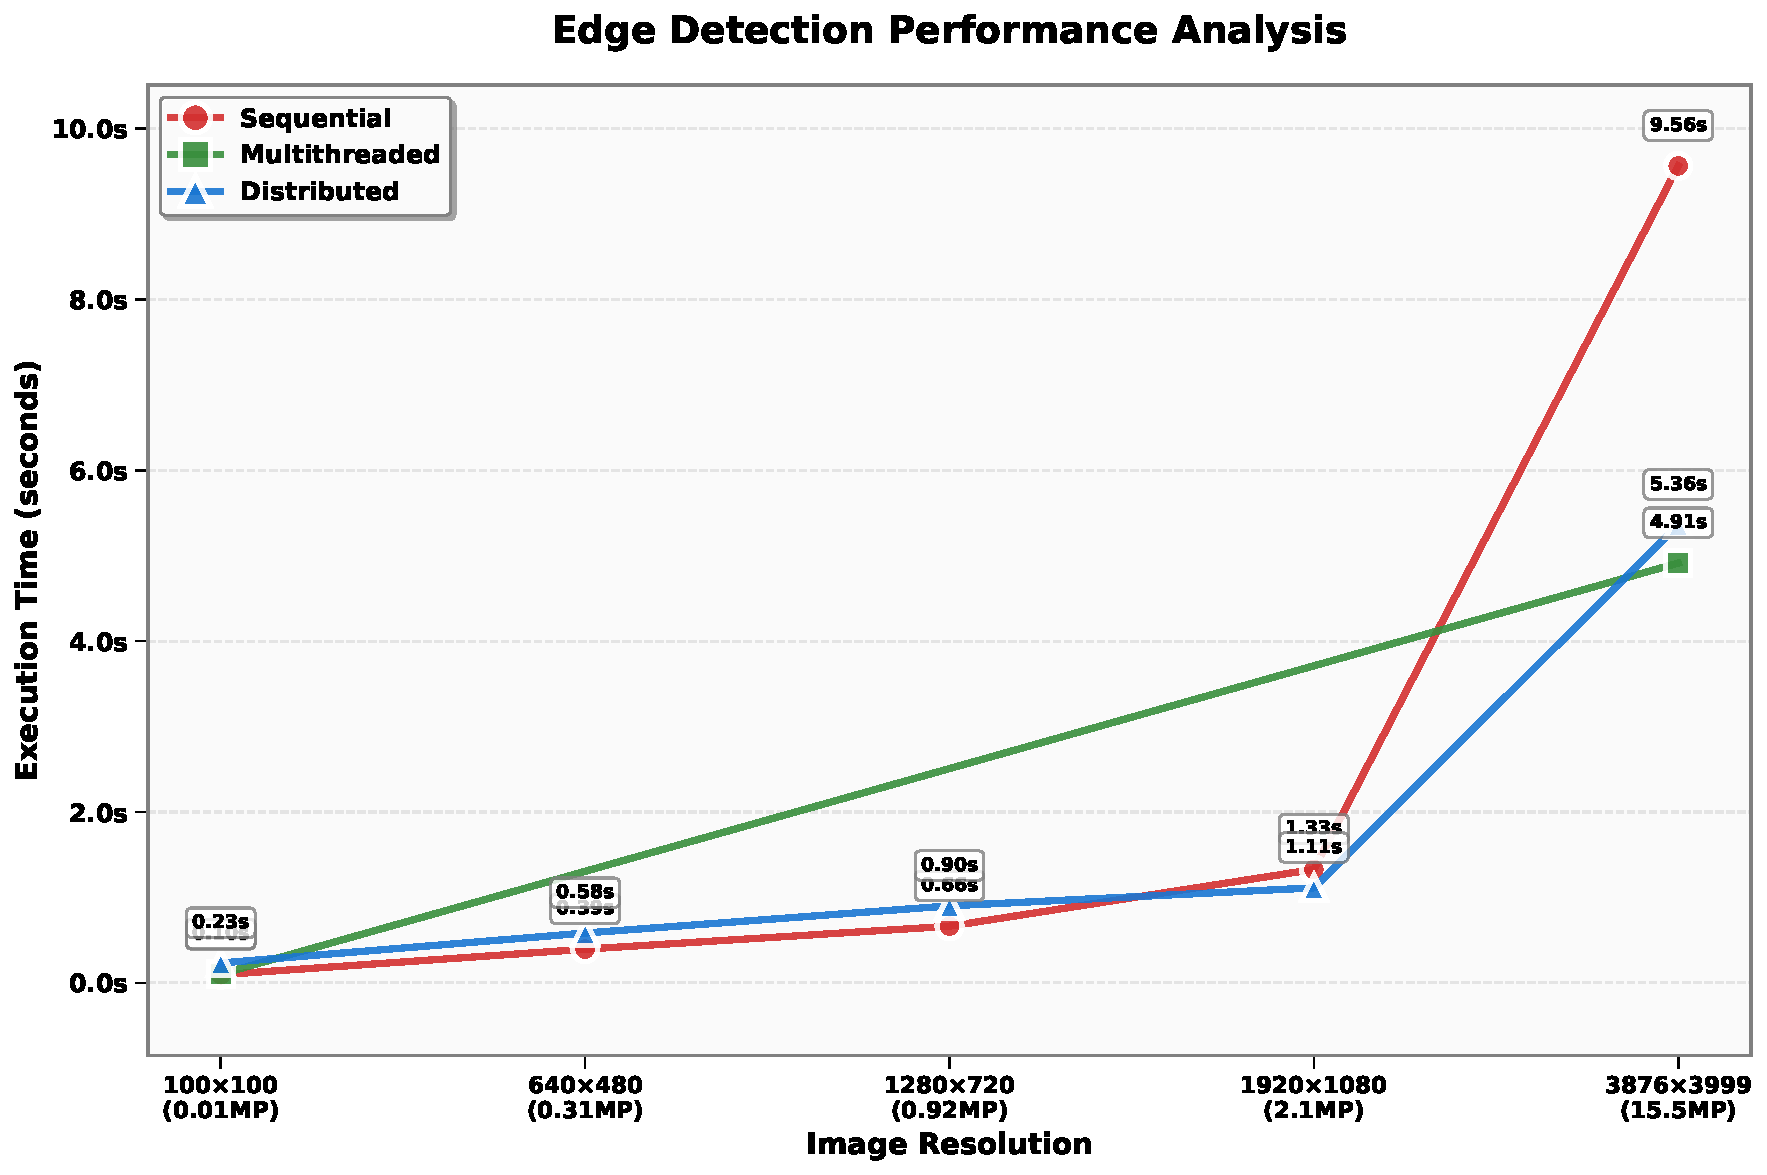
\includegraphics[width=0.9\textwidth]{graphs/edge_detection_performance.pdf}
    \caption{Edge Detection: Performance analysis across different image sizes}
    \label{fig:edge_detection_performance}
\end{figure}

\subsection{Blur Filter Performance}
\begin{figure}[htbp]
    \centering
    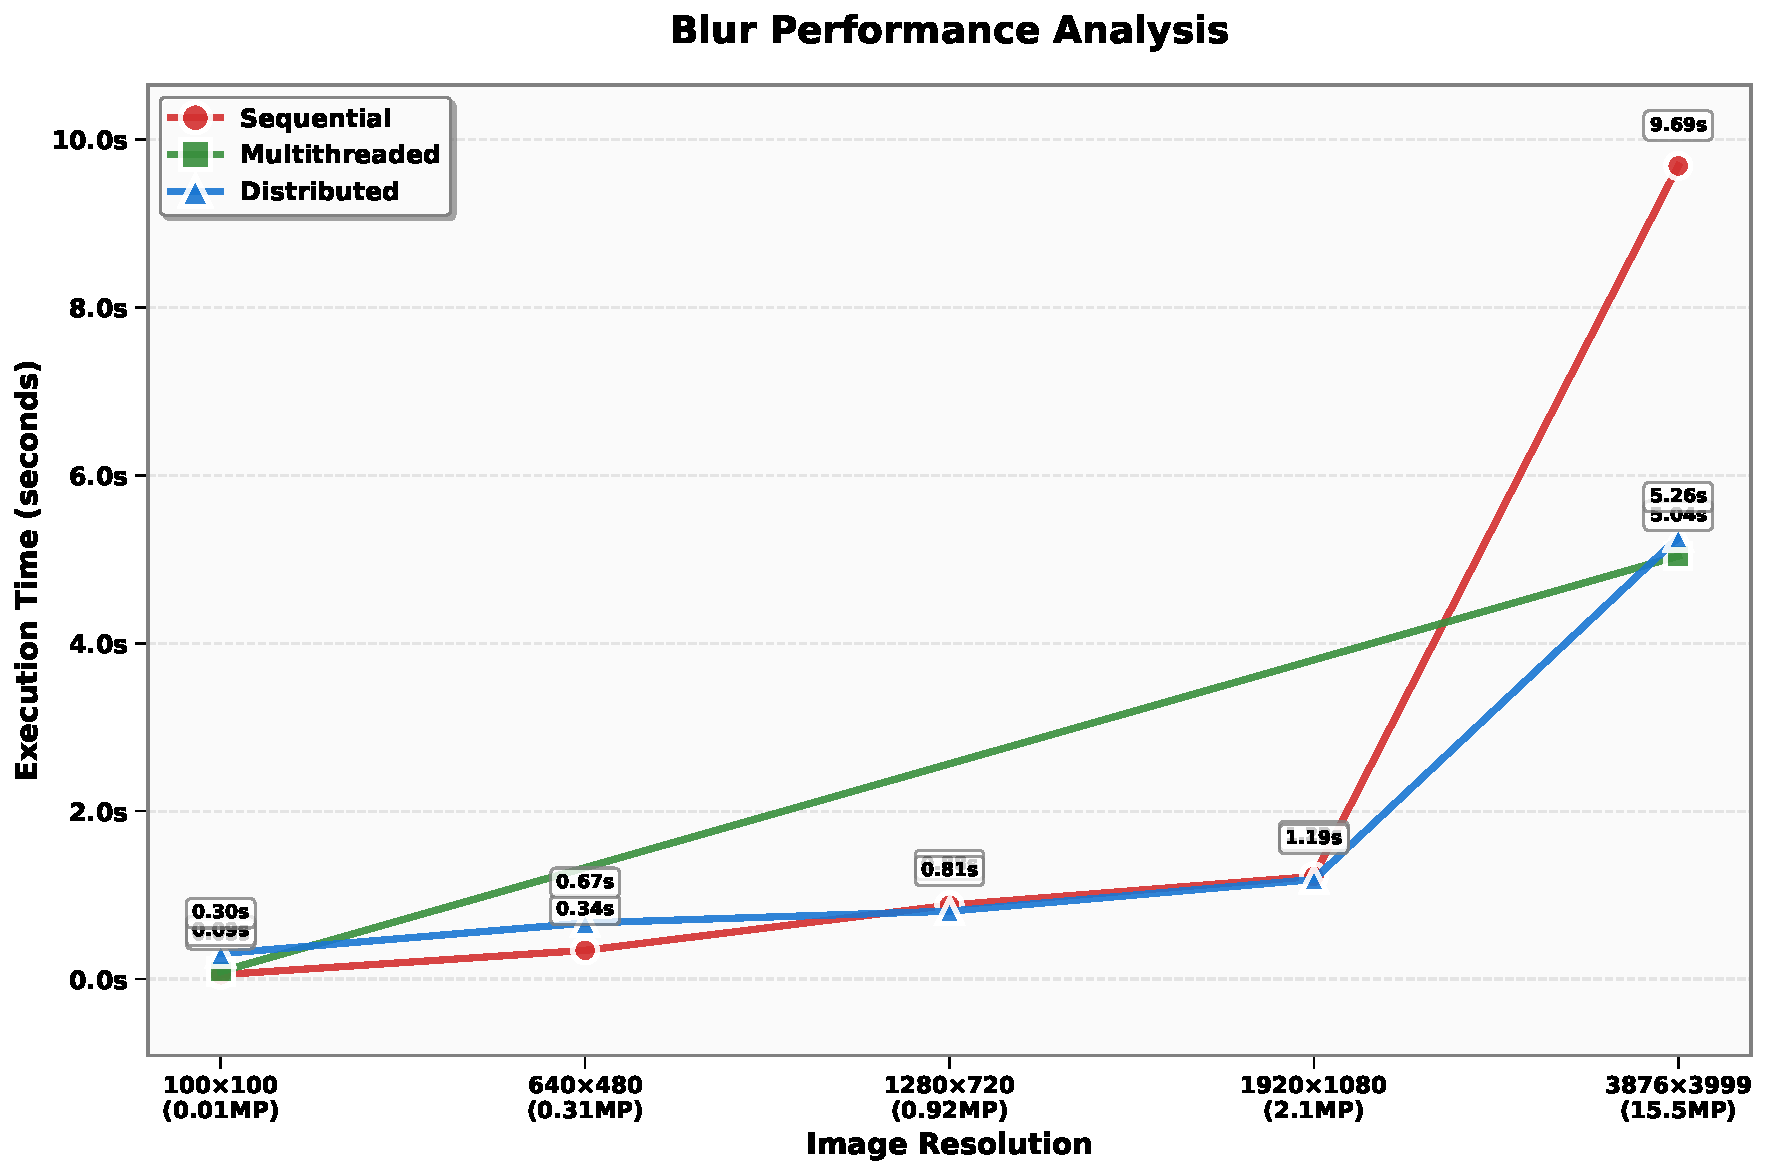
\includegraphics[width=0.9\textwidth]{graphs/blur_performance.pdf}
    \caption{Blur Filter: Performance analysis across different image sizes}
    \label{fig:blur_performance}
\end{figure}

\subsection{Sharpen Filter Performance}
\begin{figure}[htbp]
    \centering
    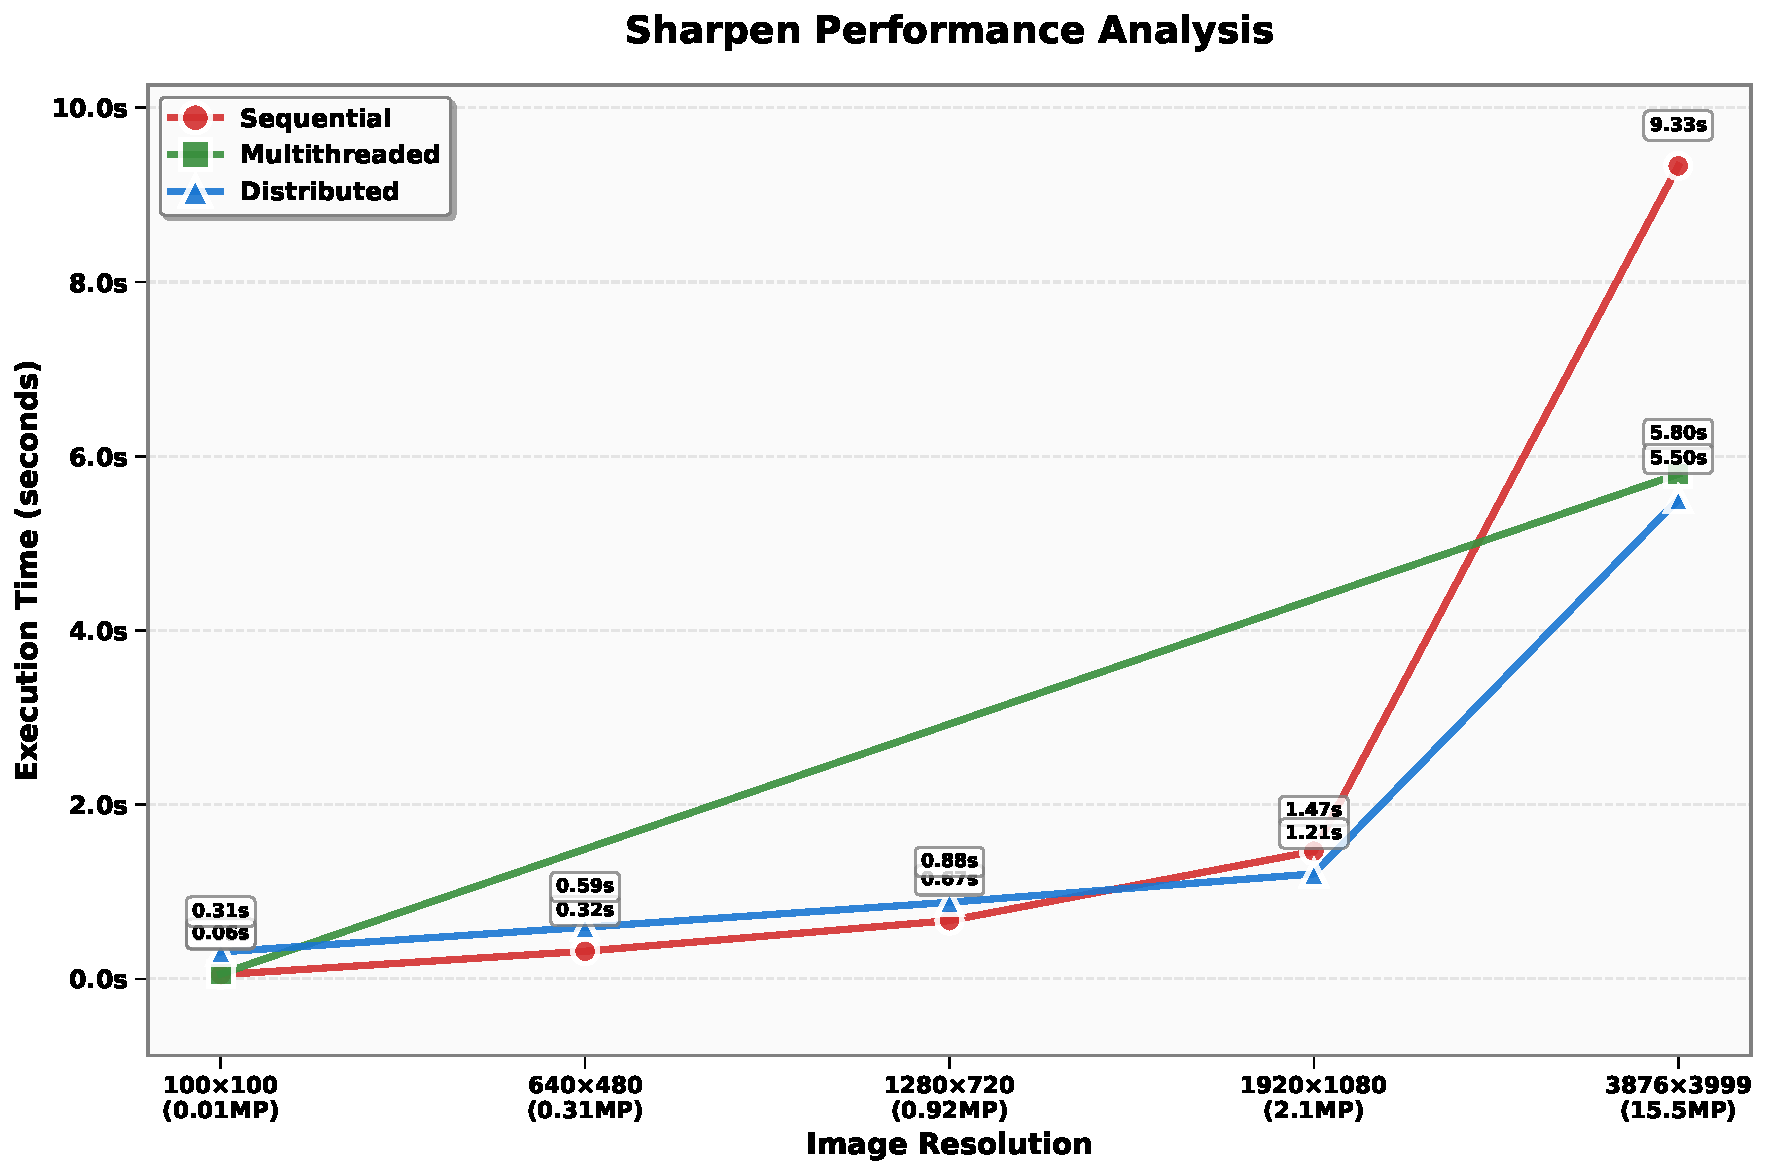
\includegraphics[width=0.9\textwidth]{graphs/sharpen_performance.pdf}
    \caption{Sharpen Filter: Performance analysis across different image sizes}
    \label{fig:sharpen_performance}
\end{figure}

\subsection{Performance Speedup Summary}
\begin{figure}[htbp]
    \centering
    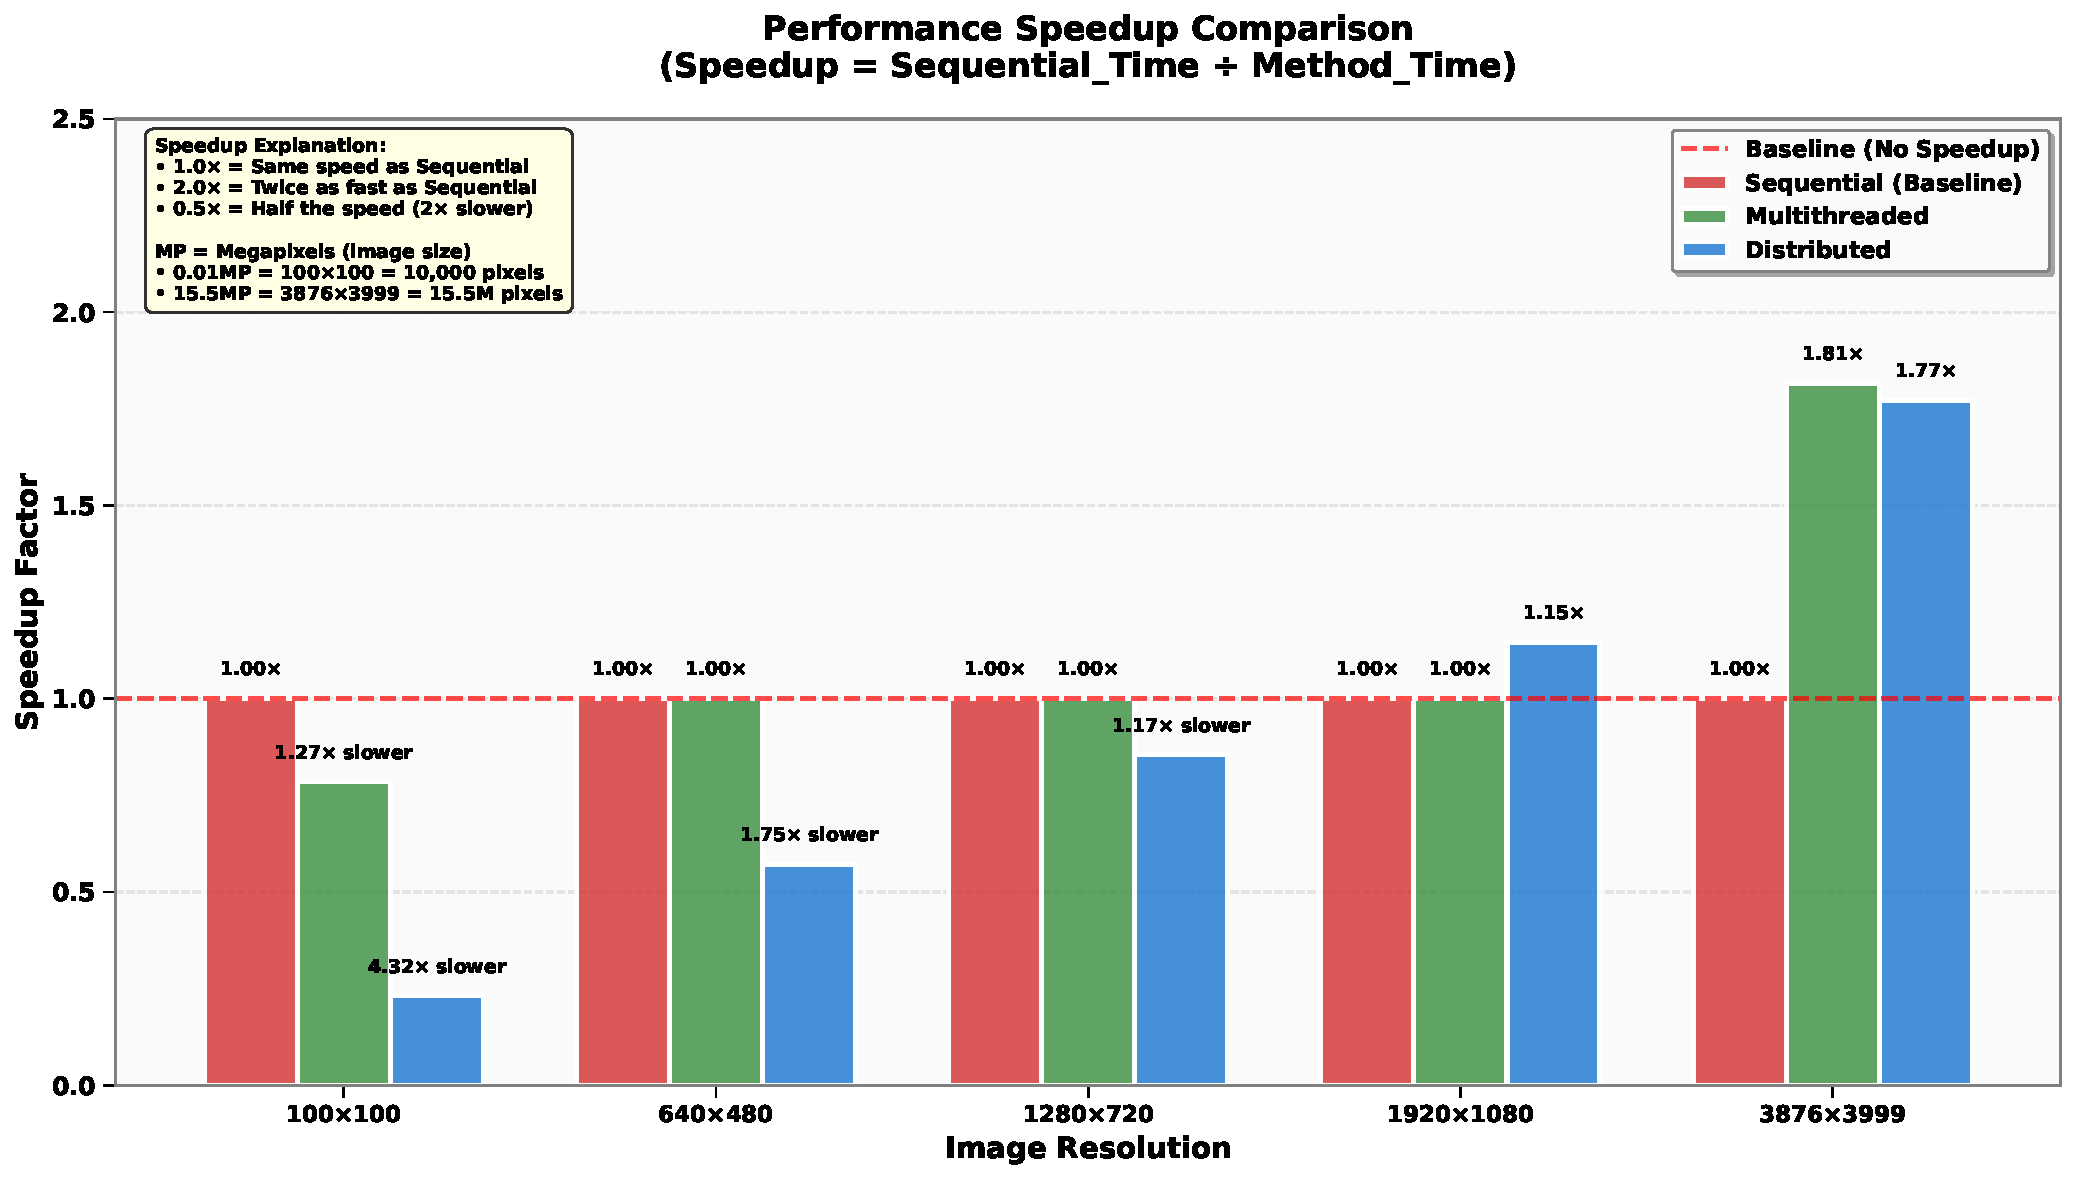
\includegraphics[width=0.9\textwidth]{graphs/speedup_summary.pdf}
    \caption{Performance speedup comparison: Multithreaded and Distributed vs Sequential processing}
    \label{fig:speedup_summary}
\end{figure}
